\chapter{Klasser}
En HiFi-forstærkers udgangstrin kan designes på forskellige måder alt efter hvilke karakteristika man ønsker at opnå. De forskellige designs er opdelt ved henhold af klassifikation. I dette afsnit vil der blive taget udgangspunkt i grundkoblinger, som viser funktionaliteten af de forsk 
I dette afsnit vil der blive gjort rede for de gængse klassifikationer, som har med analogt opbyggede forstærkere at gøre, og forklare hvilke fordele og ulemper der er med dem. Der vil, på baggrund af dette afsnit, blive valgt en endelig udgangstrinsklasse til dette projekts HiFi-forstærker hvilket vil blive opstillet, som et krav i kravspecifikationen.

\section{Klasse A}

En klasse A forstærker er opbygget af to NPN transistorer, Q1 og Q2, i en emitterfølgerkobling, som vist på figur \ref{fig:classa}. Inputsignalet kommer ind på Q1's base og styrer således strømmen der kan løbe gennem Q1 og loadmodstanden. 

\begin{figure}[h]
\centering
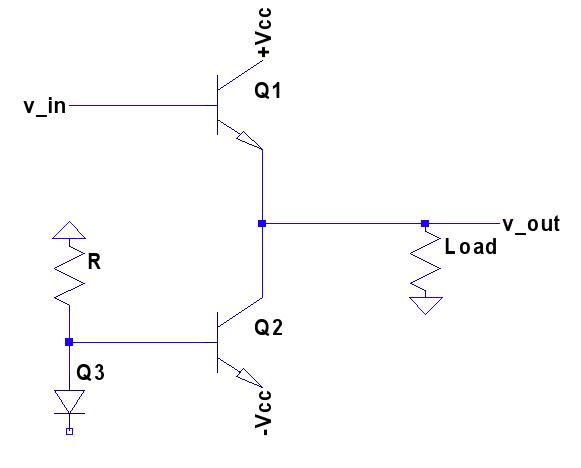
\includegraphics[scale=.6]{klasser/classa.png}
\caption{Klasse A forstærker kredsløb.}
\label{fig:classa}
\end{figure}


\section{Klasse B}
En klasse B forstærker er opbygget af to transistorer, en NPN (Q1) og en PNP (Q2), som vist på figur \ref{fig:classb}. Når input spændingen overstiger ca. 0,5 V vil Q1 begynde at lede strøm til loadmodstanden mens Q2 er lukket. Kommer input spændingen under -0,5 V vil Q2 lede, men da Q2 er en PNP vil den trække strøm mod -Vcc hvormed der trækkes strøm fra loadmodstanden. Når Q2 leder er Q1 lukket. 
Der afsættes ikke nær så meget effekt i en klasse B forstærker når input spændingen er 0 V, som i en klasse A. Dette skyldes at klasse B har et dødområde, grundet transistorerne saturation-spænding. Dødområdet er, i ovenstående eksempel, på +-0,5 V. 

\begin{figure}[h]
\centering
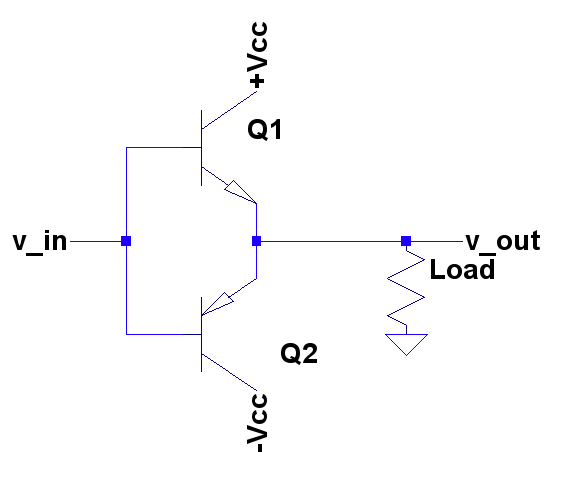
\includegraphics[scale=.6]{klasser/classb.png}
\caption{Klasse B forstærker kredsløb.}
\label{fig:classb}
\end{figure}

\section{Klasse AB}
\begin{figure}[h]
\centering
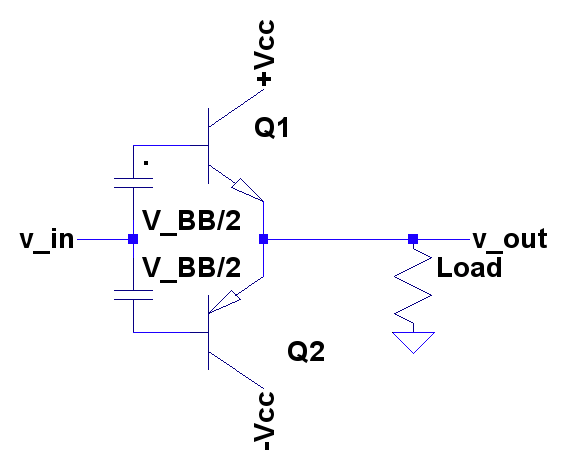
\includegraphics[scale=.6]{klasser/classab.png}
\caption{Klasse AB forstærker kredsløb.}
\label{fig:classab}
\end{figure}